\documentclass[11pt]{article}

\usepackage[margin=1in]{geometry}
\usepackage{amsmath,amssymb,amsthm}
\usepackage{mathtools}
\usepackage{enumitem}
\usepackage{tikz}
\usepackage[hidelinks]{hyperref}

\title{Algorithms for Approximate Inversion of Weave Structures}
\author{Peter E. Francis}
\date{\today}

\newtheorem{definition}{Definition}
\newtheorem{theorem}{Theorem}
\newtheorem{observation}{Observation}
\newtheorem{proposition}{Proposition}
\newtheorem{example}{Example}

\begin{document}

\maketitle

\begin{abstract}
This paper studies the inverse problem for shaft-loom weaving: given a desired
binary drawdown, find a threading, tie-up, and treadling that reproduce it
exactly when possible, and approximate it well when exact reproduction is
impossible under loom constraints.
\end{abstract}

\tableofcontents
\clearpage

\section{Introduction}

A single-layer woven structure may be idealized as a binary matrix
\[
  \widehat{D} \in \{0,1\}^{p \times w},
\]
where \(p\) is the number of weft picks and \(w\) is the number of warp ends.
Rows index picks and columns index warp ends. We use the convention
\[
  \widehat{D}_{ij}
  =
  \begin{cases}
    1, & \text{warp end } j \text{ passes over weft pick } i,\\
    0, & \text{weft pick } i \text{ passes over warp end } j.
  \end{cases}
\]
In this language, a Jacquard loom is essentially unconstrained: each warp end
may be controlled independently on each pick, so every finite binary matrix is
attainable, ignoring physical considerations such as yarn behavior, abrasion,
float length, and cloth stability. Matrix and algebraic models of loom
constraints go back at least to Lourie's work on loom-constrained designs, which
represents a weave as a binary matrix and studies how to recover loom data from
that matrix~\cite{lourie1969}.

The situation is very different for a shaft loom. A warp end is threaded through
one shaft, and all warp ends on the same shaft move together. Thus a shaft loom
cannot directly control individual warp ends; it controls equivalence classes of
warp ends. Let \(t\) be the number of treadles, \(s\) the number of shafts, and
\(r\) the maximum number of treadles allowed to be pressed on a single pick.
We encode a draft by three binary matrices:
\[
  A \in \{0,1\}^{p \times t},
  \qquad
  B \in \{0,1\}^{s \times t},
  \qquad
  C \in \{0,1\}^{s \times w}.
\]
Here \(A\) is the treadling matrix, with \(A_{i\ell}=1\) if treadle \(\ell\) is
pressed on pick \(i\); \(B\) is the tie-up matrix, with \(B_{h\ell}=1\) if
treadle \(\ell\) lifts shaft \(h\); and \(C\) is the threading matrix, with
\(C_{hj}=1\) if warp end \(j\) is threaded on shaft \(h\). Each column of \(C\)
contains exactly one nonzero entry, and each row of \(A\) contains at most \(r\)
nonzero entries.

\begin{figure}[ht]
  \centering
  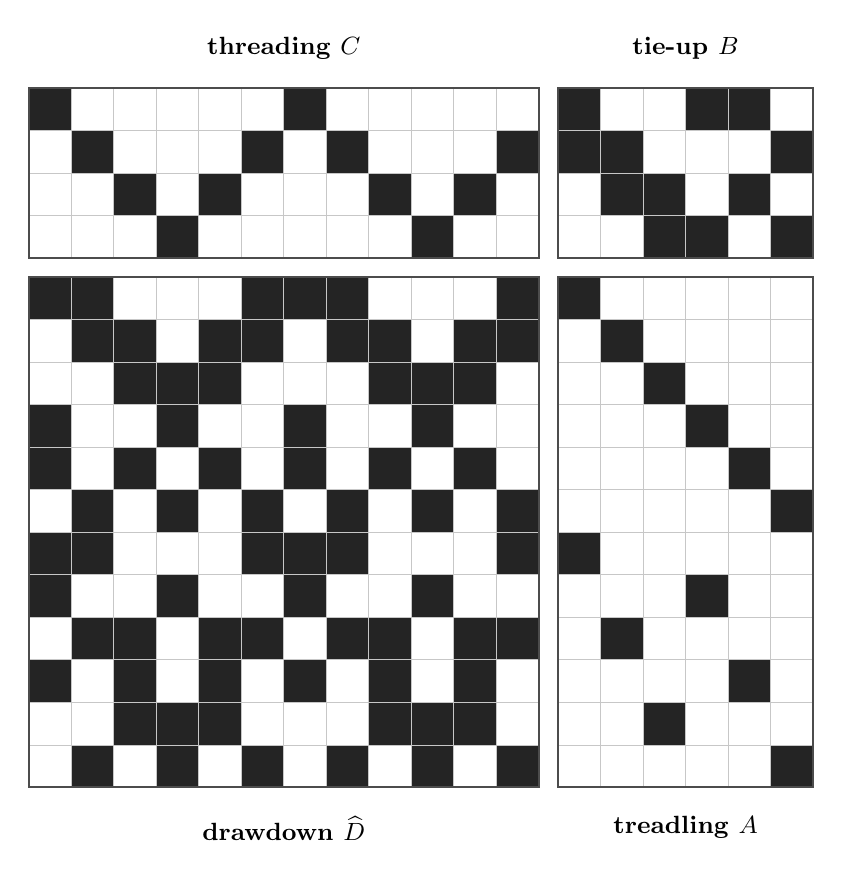
\begin{tikzpicture}[
    x=0.54cm,
    y=0.54cm,
    gridline/.style={draw=black!22, line width=0.25pt},
    sectionline/.style={draw=black!70, line width=0.7pt},
    block/.style={fill=black!86},
    label/.style={font=\small\bfseries}
  ]
    \def\gap{0.45}
    \newcommand{\sectiongrid}[2]{%
      \foreach \x in {0,...,#1} {\draw[gridline] (\x,0) -- (\x,#2);}
      \foreach \y in {0,...,#2} {\draw[gridline] (0,\y) -- (#1,\y);}
      \draw[sectionline] (0,0) rectangle (#1,#2);
    }

    \begin{scope}[shift={(0,12+\gap)}]
      \foreach \x/\y in {0/3,1/2,2/1,3/0,4/1,5/2,6/3,7/2,8/1,9/0,10/1,11/2} {
        \fill[block] (\x,\y) rectangle ++(1,1);
      }
      \sectiongrid{12}{4}
      \node[label, above] at (6,4.45) {threading \(C\)};
    \end{scope}

    \begin{scope}[shift={(12+\gap,12+\gap)}]
      \foreach \x/\y in {0/3,0/2,1/2,1/1,2/1,2/0,3/0,3/3,4/3,4/1,5/2,5/0} {
        \fill[block] (\x,\y) rectangle ++(1,1);
      }
      \sectiongrid{6}{4}
      \node[label, above] at (3,4.45) {tie-up \(B\)};
    \end{scope}

    \begin{scope}
      \foreach \x/\y in {
        0/11,1/11,5/11,6/11,7/11,11/11,
        1/10,2/10,4/10,5/10,7/10,8/10,10/10,11/10,
        2/9,3/9,4/9,8/9,9/9,10/9,
        0/8,3/8,6/8,9/8,
        0/7,2/7,4/7,6/7,8/7,10/7,
        1/6,3/6,5/6,7/6,9/6,11/6,
        0/5,1/5,5/5,6/5,7/5,11/5,
        0/4,3/4,6/4,9/4,
        1/3,2/3,4/3,5/3,7/3,8/3,10/3,11/3,
        0/2,2/2,4/2,6/2,8/2,10/2,
        2/1,3/1,4/1,8/1,9/1,10/1,
        1/0,3/0,5/0,7/0,9/0,11/0
      } {
        \fill[block] (\x,\y) rectangle ++(1,1);
      }
      \sectiongrid{12}{12}
      \node[label, below] at (6,-0.45) {drawdown \(\widehat{D}\)};
    \end{scope}

    \begin{scope}[shift={(12+\gap,0)}]
      \foreach \x/\y in {0/11,1/10,2/9,3/8,4/7,5/6,0/5,3/4,1/3,4/2,2/1,5/0} {
        \fill[block] (\x,\y) rectangle ++(1,1);
      }
      \sectiongrid{6}{12}
      \node[label, below] at (3,-0.45) {treadling \(A\)};
    \end{scope}
  \end{tikzpicture}
  \caption{A draft written as matrices.  Dark cells are entries equal to \(1\).
  This example uses \(w=p=12\), \(s=4\), and \(t=6\): the threading \(C\),
  tie-up \(B\), and treadling \(A\) determine the drawdown by thresholding the
  redundancy matrix \(D=AB^TC\).}
  \label{fig:example-draft}
\end{figure}

The natural product in this notation is
\[
  D = A B^{T} C.
\]
The matrix \(D\) is not merely binary. It records the redundancy with which each
cell is activated.

\begin{theorem}[Redundancy matrix]
Let \(A\in\{0,1\}^{p\times t}\) be a treadling matrix, let
\(B\in\{0,1\}^{s\times t}\) be a tie-up matrix, and let
\(C\in\{0,1\}^{s\times w}\) be a threading matrix with exactly one nonzero entry
in each column. Define
\[
  D = A B^{T} C.
\]
Then \(D\in\mathbb{Z}_{\ge 0}^{p\times w}\), and \(D_{ij}\) is the number of
pressed treadles on pick \(i\) that lift the shaft containing warp end \(j\).
In particular, if
\[
  \widehat{D}_{ij}=\mathbf{1}\{D_{ij}>0\},
\]
then \(\widehat{D}_{ij}=1\) exactly when warp end \(j\) is lifted over pick
\(i\). Moreover, if at most \(r\) treadles are pressed on each pick, then
\[
  0 \le D_{ij} \le r
  \qquad
  \text{for all } i,j.
\]
\end{theorem}

\begin{proof}
By the definition of matrix multiplication,
\[
  D_{ij}
  =
  (AB^{T}C)_{ij}
  =
  \sum_{\ell=1}^{t}\sum_{h=1}^{s} A_{i\ell}B_{h\ell}C_{hj}.
\]
Since warp end \(j\) is threaded on exactly one shaft, there is a unique shaft
\(h(j)\) such that \(C_{h(j),j}=1\), and \(C_{hj}=0\) for \(h\ne h(j)\).
Therefore the double sum collapses to
\[
  D_{ij}
  =
  \sum_{\ell=1}^{t} A_{i\ell}B_{h(j),\ell}.
\]
For a fixed pick \(i\), the factor \(A_{i\ell}\) is \(1\) exactly when treadle
\(\ell\) is pressed. The factor \(B_{h(j),\ell}\) is \(1\) exactly when treadle
\(\ell\) lifts the shaft \(h(j)\) carrying warp end \(j\). Thus each summand is \(1\)
exactly for a pressed treadle that lifts the shaft containing warp end \(j\), and
is \(0\) otherwise. Hence \(D_{ij}\) counts those treadles.

It follows that \(D_{ij}>0\) exactly when at least one pressed treadle lifts the
shaft containing warp end \(j\). This is precisely the event that warp end \(j\)
is lifted over pick \(i\), so the binary drawdown is
\(\widehat{D}_{ij}=\mathbf{1}\{D_{ij}>0\}\). Finally, if at most \(r\) treadles
are pressed on pick \(i\), then at most \(r\) terms in
\(\sum_{\ell=1}^{t} A_{i\ell}B_{h(j),\ell}\) can be nonzero, so \(D_{ij}\le r\).
\end{proof}

This is not ordinary unconstrained matrix factorization; it is a discrete
factorization through treadle, shaft, and warp-thread incidence matrices. Given
a target drawdown \(D^\ast\in\{0,1\}^{p\times w}\), the exact inverse problem is
to decide whether there exist admissible matrices \(A,B,C\) such that
\[
  D^\ast_{ij}=\mathbf{1}\{(AB^TC)_{ij}>0\}.
\]
When no such draft exists under the bounds \(s,t,r\), the approximate inverse
problem is to choose admissible draft matrices that minimize an objective
\[
  \Phi(\widehat{D},D^\ast;A,B,C),
  \qquad
  \widehat{D}_{ij}=\mathbf{1}\{(AB^T C)_{ij}>0\}.
\]
The functional \(\Phi\) describes the criterion by which an approximation is
judged.

A natural first objective, and the one used by the Alpha algorithms below, is
Hamming error $\Phi=\operatorname{err}$,
\[
  \operatorname{err}(\widehat{D},D^\ast)
  =
  \#\{(i,j) : \widehat{D}_{ij} \ne D^\ast_{ij}\},
\]
but the search process is still sensitive to where errors occur. Even when two
candidate drafts have the same Hamming error, a wrong cell that changes a rare
row behavior, a rare column behavior, or a local boundary may affect the
subsequent co-clustering differently from a wrong cell in a large homogeneous
region. Alpha 2 and Alpha 3 below treat such quantities as heuristics for
guiding the optimization, not as changes to the objective \(\Phi\). Separate
objectives could also penalize long warp or weft floats, disconnected prefabric
behavior, or other non-clothlike structures, but those are not part of the Alpha
objective here.

The purpose of this paper is to develop and compare algorithms for approximate
inversion. The central questions are:
\begin{enumerate}[label=(\roman*)]
  \item how to find exact factorizations when they exist;
  \item how to search efficiently when the target exceeds the available loom
  constraints;
  \item how cell-impact and redundancy heuristics can guide the search while
  retaining Hamming error as the primary objective;
  \item how to incorporate clothlike constraints such as float tolerance; and
  \item how to test an inversion engine using targets known to be generated by
  random drafts as well as targets generated by random binary drawdowns.
\end{enumerate}

\subsection*{History and context}

There are two closely related mathematical traditions behind this note. The
first is the algebraic and algorithmic analysis of weave drafts. Lourie's
``loom-constrained designs'' paper formulates the problem of determining a loom
mechanism, threading-like initial conditions, and dynamic control information
from a binary representation of a weave~\cite{lourie1969}. Hoskins and Hoskins
studied matrix equations and factoring algorithms arising from structural
analysis of woven fabrics~\cite{hoskins1981,hoskins1983}, while later work on
binary interlacement arrays and bounded-float twills develops related finite
combinatorial models~\cite{hoskins1984,hpstreet1983}.

The second tradition is the geometry and symmetry theory of fabrics and
prefabrics. Gr\"unbaum and Shephard introduced the modern mathematical
treatment of satins, twills, prefabrics, and isonemal fabrics
\cite{grunbaum1980,grunbaum1985,grunbaum1986,grunbaum1988}. Roth classified the
symmetry groups of periodic isonemal fabrics~\cite{roth1993}, and Thomas
refined Roth's taxonomy for prefabrics with parallel axes, perpendicular axes,
and no axes of symmetry~\cite{thomas2009,thomas2010perp,thomas2010noaxes}.
Questions about whether a prefabric ``hangs together'' are separate from
symmetry classification and lead to their own graph-like connectivity
criteria~\cite{clapham1980,delaney1986,enns1984}.

The present paper uses the same binary-matrix language, but focuses on a slightly
different computational question: when an exact shaft-loom factorization is
unavailable or undesirable, how should one approximate the target drawdown? In
particular, we keep track of the integer redundancy matrix \(D=AB^TC\), allow
multiple treadles to be pressed on a pick, and compare search heuristics and
secondary diagnostics that may value visual locality, motif continuity, or
clothlike float behavior differently from raw Hamming error.

\section{Exact Solvability}

\begin{proposition}[Finite shaft-loom attainability with multiple treadles]
Let \(E\in\{0,1\}^{p\times w}\) be a finite binary drawdown. Delete duplicate
columns of \(E\), and call the resulting matrix \(E_{\mathrm{col}}\). Let
\(s_0\) be the number of columns of \(E_{\mathrm{col}}\), and let
\(\mathcal{R}\subseteq\{0,1\}^{s_0}\) be the set of distinct rows of
\(E_{\mathrm{col}}\).

For a set \(\mathcal{B}\subseteq\{0,1\}^{s_0}\), define its
\(r\)-fold union closure by
\[
  \mathcal{U}_r(\mathcal{B})
  =
  \left\{
    b_1\vee b_2\vee\cdots\vee b_k
    :
    0\le k\le r,\ b_1,\dots,b_k\in\mathcal{B}
  \right\},
\]
where \(\vee\) denotes coordinatewise Boolean OR and the empty union is the
zero vector. Then \(E\) is attainable on a shaft loom with at most \(s\) shafts,
\(t\) treadles, and at most \(r\) treadles pressed on any pick if and only if
\[
  s_0\le s
  \qquad\text{and}\qquad
  \mathcal{R}\subseteq \mathcal{U}_r(\mathcal{B})
\]
for some set \(\mathcal{B}\subseteq\{0,1\}^{s_0}\) with
\(|\mathcal{B}|\le t\).

When \(r=1\) and each pick is required to use a single treadle, this reduces to
the simpler criterion that the reduced drawdown has at most \(s\) distinct
column types and at most \(t\) distinct row types. With enough treadles or with a
dobby-style liftplan, the minimum number of shafts is the number of distinct
warp-column behaviors. For an infinite periodic prefabric, the same criterion
applies to a fundamental period block.
\end{proposition}

\begin{proof}
First suppose that \(E\) is produced by a shaft loom with at most \(s\) shafts,
\(t\) treadles, and at most \(r\) treadles pressed on a pick. If two warp ends
are threaded on the same shaft, then they are lifted on exactly the same picks,
so their columns in \(E\) are identical. Therefore the number of distinct column
behaviors is at most the number of shafts, hence \(s_0\le s\).

After duplicate columns are removed, each treadle determines a binary vector in
\(\{0,1\}^{s_0}\): its entries record which of the \(s_0\) column types are
lifted by that treadle. Let \(\mathcal{B}\) be the set of these treadle vectors.
Then \(|\mathcal{B}|\le t\). If pick \(i\) presses treadles
\(\ell_1,\dots,\ell_k\), with \(k\le r\), then its reduced row is the Boolean union
of the corresponding treadle vectors,
\[
  b_{\ell_1}\vee\cdots\vee b_{\ell_k}.
\]
Thus every distinct reduced row lies in \(\mathcal{U}_r(\mathcal{B})\).

Conversely, suppose \(s_0\le s\) and
\(\mathcal{R}\subseteq\mathcal{U}_r(\mathcal{B})\) for some
\(\mathcal{B}=\{b_1,\dots,b_m\}\subseteq\{0,1\}^{s_0}\) with \(m\le t\).
Assign each distinct column type to one shaft, threading every warp end with
that column behavior through the corresponding shaft. Assign the vector
\(b_\ell\) to treadle \(\ell\), tying it to exactly those shafts whose column types
have value \(1\) in \(b_\ell\). Since every reduced row of \(E\) is a Boolean union
of at most \(r\) vectors from \(\mathcal{B}\), choose one such representation
for each pick and press the corresponding treadles. The resulting thresholded
drawdown is exactly \(E\).

For \(r=1\), each reduced row must itself be one of the treadle vectors, so the
criterion reduces to counting distinct reduced row types. If pressing no treadle
is disallowed, one simply omits the empty union from
\(\mathcal{U}_r(\mathcal{B})\).

For a periodic prefabric, all rows and columns are determined by a finite
fundamental period block, so applying the same argument to that block gives the
periodic statement.
\end{proof}

Thus, when \(r>1\), the minimum number of treadles is no longer simply the
number of distinct reduced row types. It is the size of the smallest family of
basic treadle lift patterns whose Boolean unions of size at most \(r\) cover all
reduced row types.

\subsection*{Exact recovery algorithm}

The proposition gives a direct complete algorithm for recovering a draft
\((A,B,C)\) from a target drawdown \(\widehat{D}\), if such a draft exists under
the size constraints. The algorithm starts from \(\mathcal{R}\), because after
duplicate warp-column behaviors are removed, \(\mathcal{R}\) is equivalent to
the target for the purpose of deciding which treadle lift patterns are needed.
Repeated picks only repeat rows of \(A\), and repeated warp-column behaviors
only repeat columns of \(C\).

\paragraph{Input.}
A target drawdown \(\widehat{D}\in\{0,1\}^{p\times w}\), a shaft bound \(s\), a
treadle bound \(t\), and a maximum number \(r\) of treadles pressed on a pick.

\paragraph{Step 1: recover the threading.}
Group the columns of \(\widehat{D}\) by equality. Let
\[
  c(j)\in\{1,\dots,s_0\}
\]
be the column class of warp end \(j\), and let \(s_0\) be the number of distinct
column classes. If \(s_0>s\), stop: no draft with at most \(s\) shafts exists.
Otherwise define \(C\in\{0,1\}^{s\times w}\) by
\[
  C_{h j}
  =
  \begin{cases}
    1, & h=c(j),\\
    0, & \text{otherwise}.
  \end{cases}
\]
Unused shafts \(s_0+1,\dots,s\) are left empty.

\paragraph{Step 2: reduce to row types.}
Delete duplicate column classes from \(\widehat{D}\) to obtain
\[
  E_{\mathrm{col}}\in\{0,1\}^{p\times s_0}.
\]
Let \(\mathcal{R}\subseteq\{0,1\}^{s_0}\) be the set of distinct rows of
\(E_{\mathrm{col}}\). For each pick \(i\), record its reduced row type
\[
  q(i)\in\mathcal{R}.
\]
At this point the remaining problem is equivalent to finding treadle generators
whose Boolean unions produce the rows in \(\mathcal{R}\).

\paragraph{Step 3: solve the generator problem.}
Form the finite candidate set
\[
  \mathcal{C}
  =
  \{b\in\{0,1\}^{s_0}: b\le q \text{ coordinatewise for some }
  q\in\mathcal{R}\}.
\]
Search over subsets \(\mathcal{B}\subseteq\mathcal{C}\) with
\(|\mathcal{B}|\le t\). For each candidate \(\mathcal{B}\), compute
\(\mathcal{U}_r(\mathcal{B})\). If
\[
  \mathcal{R}\subseteq\mathcal{U}_r(\mathcal{B}),
\]
then choose, for every row type \(q\in\mathcal{R}\), a representation
\[
  q=b_{\ell_1}\vee\cdots\vee b_{\ell_k},
  \qquad
  k\le r,
  \qquad
  b_{\ell_1},\dots,b_{\ell_k}\in\mathcal{B}.
\]
If no such \(\mathcal{B}\) exists, stop: no draft with the prescribed
\((s,t,r)\) constraints exists.

\paragraph{Step 4: recover the tie-up and treadling.}
Index the selected generators as
\[
  \mathcal{B}=\{b_1,\dots,b_m\},
  \qquad
  m\le t.
\]
Define \(B\in\{0,1\}^{s\times t}\) by
\[
  B_{h \ell}
  =
  \begin{cases}
    (b_\ell)_h, & 1\le h\le s_0,\ 1\le \ell\le m,\\
    0, & \text{otherwise}.
  \end{cases}
\]
For each pick \(i\), use the chosen representation of \(q(i)\) and set
\[
  A_{i \ell}
  =
  \begin{cases}
    1, & b_\ell \text{ is used in the chosen representation of } q(i),\\
    0, & \text{otherwise}.
  \end{cases}
\]
Then each row of \(A\) has at most \(r\) nonzero entries.

\begin{proposition}[Correctness of exact recovery]
The algorithm above returns matrices \(A,B,C\) satisfying
\[
  \widehat{D}_{ij}
  =
  \mathbf{1}\{(AB^TC)_{ij}>0\}
\]
whenever such matrices exist under the constraints \(s,t,r\). If the algorithm
reports failure, no such draft exists.
\end{proposition}

\begin{proof}
Step 1 is forced: warp ends with different columns in \(\widehat{D}\) cannot be
threaded on the same shaft, since shafts move their warp ends together. Thus
any exact draft must use at least \(s_0\) shafts, and grouping equal columns
loses no information.

After this reduction, each treadle corresponds to a vector in
\(\{0,1\}^{s_0}\), recording which column classes it lifts. If a treadle vector
appears in a union producing a row \(q\), then it must be coordinatewise
contained in \(q\). Therefore every useful treadle vector lies in the candidate
set \(\mathcal{C}\); vectors outside \(\mathcal{C}\) either cannot be used or
would lift a shaft in a row where it should remain unlifted.

Thus an exact draft exists precisely when there is a set
\(\mathcal{B}\subseteq\mathcal{C}\) of at most \(t\) treadle vectors such that
every reduced row type in \(\mathcal{R}\) is a Boolean union of at most \(r\)
vectors from \(\mathcal{B}\). Step 3 searches this finite space exhaustively, so
it finds such a family if one exists and fails only if none exists.

Given such a family, Step 4 makes \(B\) from the selected generators and makes
\(A\) from the chosen union representation of each pick. By construction, the
thresholded product \(AB^TC\) reproduces every reduced row on the corresponding
column classes, and \(C\) then repeats those column classes across the original
warp ends. Therefore the thresholded drawdown is exactly \(\widehat{D}\).
\end{proof}

The periodic version of this statement uses the language of prefabrics and
fabrics, which we recall here.

\begin{definition}[Prefabric]
A \emph{prefabric} is a formal infinite over-under assignment for two transverse
families of strands, one warp-like and one weft-like. A prefabric need not hang
together as a physical cloth; it may fall apart into independent layers, strips,
or components~\cite{grunbaum1980,clapham1980,enns1984}.
\end{definition}

\begin{definition}[Fabric and isonemal fabric]
A \emph{fabric} is a prefabric whose strands interlace sufficiently to hang
together. A fabric is \emph{isonemal} if its symmetry group acts transitively on
the set of strands; equivalently, for any two strands, there is a symmetry of
the fabric that sends one strand to the other~\cite{grunbaum1980,grunbaum1988}.
\end{definition}

The symmetry theory of periodic fabrics, including isonemal fabrics, is largely
orthogonal to shaft attainability. A design can be highly symmetric and still
require many shaft-column behaviors. Conversely, a design can be attainable on
few shafts while failing to be a good physical cloth because of floats,
instability, or other textile constraints.

\section{Alpha Algorithms (Hamming Error)}

The Alpha algorithms are the approximate engines obtained by instantiating
\(\Phi\) with the Hamming weight of the binary discrepancy pattern
\(\Delta(\widehat{D},D^\ast)=\widehat{D}\oplus D^\ast\). For Alpha 1, Alpha 2,
and Alpha 3, the primary objective is the raw Hamming weight
\(\sum_{i,j}\Delta_{ij}\), so every cell disagreement has equal final cost.
The difference between the methods is algorithmic rather than objective:
Alpha 1 is the baseline co-clustering search, Alpha 2 adds cell-impact search
pressure, and Alpha 3 adds redundancy search pressure. The later variants are
not defined merely to be non-worsening wrappers around the earlier ones. They
are allowed to change the search dynamics, and their justification is empirical:
they should lower the average optimality gap under the same final Hamming
objective.

\subsection{Alpha 1}
When the exact problem fails under the prescribed bounds
\(s,t,r\), the first approximation method, called \emph{Alpha 1}, replaces the
union-closure search by a finite binary co-clustering problem. Alpha 1 is the
baseline member of the Alpha family: it uses ordinary Hamming disagreement
throughout the co-clustering search and should be regarded as the reference
approximation algorithm.

Let
\[
  \tau:\{1,\dots,p\}\to\{1,\dots,t'\},
  \qquad
  \chi:\{1,\dots,w\}\to\{1,\dots,s'\}
\]
be row and column assignments, with \(t'\le t\) and \(s'\le s\). The map
\(\tau\) assigns picks to provisional treadle states, while \(\chi\) assigns
warp ends to provisional shaft states. For a reduced tie-up
\[
  U\in\{0,1\}^{t'\times s'},
\]
the corresponding approximate drawdown is
\[
  \widehat{D}_{ij}=U_{\tau(i),\chi(j)}.
\]
Alpha 1 approximately minimizes the co-clustering loss
\[
  L_0(\tau,\chi,U)
  =
  \sum_{i=1}^{p}\sum_{j=1}^{w}
  \mathbf{1}\{U_{\tau(i),\chi(j)}\ne D^\ast_{ij}\}.
\]
This objective is not the original shaft-loom problem, because it ignores the
multi-treadle union representation while the clustering is being optimized. It
is instead a tractable relaxation that is subsequently converted back into
draft matrices \(A,B,C\).

\begin{proposition}[Majority tie-up update]
Fix assignments \(\tau\) and \(\chi\). A minimizer of
\(L_0(\tau,\chi,U)\) over \(U\in\{0,1\}^{t'\times s'}\) is obtained entrywise
by
\[
  U_{ab}
  =
  \begin{cases}
    1,
    &
    \displaystyle
    \sum_{i:\tau(i)=a}\sum_{j:\chi(j)=b}D^\ast_{ij}
    \ge
    \frac{1}{2}
    \#\{(i,j):\tau(i)=a,\ \chi(j)=b\},
    \\[1.2em]
    0, & \text{otherwise}.
  \end{cases}
\]
\end{proposition}

\begin{proof}
For fixed \(a\) and \(b\), the entry \(U_{ab}\) affects only the block of cells
\((i,j)\) satisfying \(\tau(i)=a\) and \(\chi(j)=b\). Choosing \(U_{ab}=0\)
incurs exactly one error for each \(1\) in that block, while choosing
\(U_{ab}=1\) incurs exactly one error for each \(0\) in that block. Hence the
optimal value is the majority value in the block. The blocks are disjoint, so
the same argument applies independently to every entry of \(U\).
\end{proof}

\subsubsection*{Procedure}

Alpha 1 is a multi-start alternating minimization procedure. It uses a finite
set \(\mathcal{I}\) of initializations, such as farthest-first, density-ordered,
and random assignments. The distance-based initializations use ordinary Hamming
distances between rows and columns of \(D^\ast\). For each choice of
\(s'\le s\), \(t'\le t\), and initialization, Alpha 1 performs the following
steps.

\begin{enumerate}[label=\textbf{A1.\arabic*.}]
  \item Initialize
  \[
    \tau:\{1,\dots,p\}\to\{1,\dots,t'\},
    \qquad
    \chi:\{1,\dots,w\}\to\{1,\dots,s'\}.
  \]

  \item With \(\tau\) and \(\chi\) fixed, set \(U\) by the majority rule in the
  preceding proposition.

  \item With \(\chi\) and \(U\) fixed, update each row assignment independently:
  \[
    \tau(i)
    \in
    \operatorname*{argmin}_{1\le a\le t'}
    \sum_{j=1}^{w}
    \mathbf{1}\{U_{a,\chi(j)}\ne D^\ast_{ij}\}.
  \]

  \item With \(\tau\) and \(U\) fixed, update each column assignment independently:
  \[
    \chi(j)
    \in
    \operatorname*{argmin}_{1\le b\le s'}
    \sum_{i=1}^{p}
    \mathbf{1}\{U_{\tau(i),b}\ne D^\ast_{ij}\}.
  \]

  \item Recompute \(U\). Stop if the triple \((\tau,\chi,U)\) has stabilized, or
  if a prescribed iteration limit has been reached; otherwise return to Step
  A1.3.
\end{enumerate}

For fixed \(s'\), \(t'\), and initialization, each update step weakly decreases
\(L_0\). Since the assignment space is finite, any run that forbids empty
retained groups eventually reaches a local optimum with respect to these
coordinate moves. The resulting reduced triple is converted into draft matrices
by assigning column clusters to shafts and row clusters, or unions of
row-cluster generators, to treadles. Candidate drafts are ranked first by
Hamming error, then by draft size and secondary structural diagnostics such as
line mismatch, blurred-field mismatch, density mismatch, and float behavior.

\subsection{Alpha 2}

Alpha 2 uses the same co-clustering framework and the same final objective
\(\Phi=\operatorname{err}\) as Alpha 1, but it is allowed to change the search
dynamics. The motivating suggestion is that two single-cell changes with the
same Hamming cost can have different algorithmic consequences: changing one cell
may merge a rare row behavior into a common row behavior, alter a rare column
behavior, or disturb a local boundary, while changing another cell may leave the
row-column organization nearly unchanged. Alpha 2 uses this information as
search pressure, not as a replacement for \(\Phi\).

Unlike a conservative ensemble version that keeps the full Alpha 1 candidate
pool, the main Alpha 2 algorithm is not guaranteed to be no worse than Alpha 1
on every instance. Its purpose is to find better candidates on average by
escaping different local optima. Final reporting and final candidate selection
still use ordinary Hamming error first.

\subsubsection*{Cell-impact scores}

For each row \(i\), let
\[
  \rho_i \in \{0,1\}^{w}
\]
be the \(i\)-th row pattern, and for each column \(j\), let
\[
  \kappa_j \in \{0,1\}^{p}
\]
be the \(j\)-th column pattern. Let \(m_{\mathrm{row}}(\rho)\) denote the
number of times row pattern \(\rho\) occurs, and let
\(m_{\mathrm{col}}(\kappa)\) denote the number of times column pattern
\(\kappa\) occurs.

For a cell \((i,j)\), let \(\rho_i^{(j)}\) be the row pattern obtained by
flipping coordinate \(j\), and let \(\kappa_j^{(i)}\) be the column pattern
obtained by flipping coordinate \(i\). Define
\[
  M_{ij}
  =
  \max\{
    m_{\mathrm{row}}(\rho_i^{(j)}),
    m_{\mathrm{col}}(\kappa_j^{(i)})
  \}.
\]
The quantity \(M_{ij}\) measures whether flipping a cell would merge the
affected row or column with an already existing behavior. Define also
\[
  \sigma_{ij}
  =
  \mathbf{1}\{m_{\mathrm{row}}(\rho_i)=1\}
  +
  \mathbf{1}\{m_{\mathrm{col}}(\kappa_j)=1\},
\]
which records whether the cell lies in a row or column behavior that occurs
only once, and let \(e_{ij}\) be the number of horizontal or vertical neighbors
of \((i,j)\) whose value differs from \(D^\ast_{ij}\). Alpha 2 assigns the
heuristic impact score
\[
  \eta_{ij}
  =
  \min\left\{
    6,
    1
    +
    \log_2(1+M_{ij})
    +
    0.35\,\sigma_{ij}
    +
    0.08\,e_{ij}
    +
    \frac{M_{ij}}{\max(p,w)}
  \right\}.
\]
The score \(\eta_{ij}\) is not part of \(\Phi\). It is a heuristic estimate of
how much row-column structure is touched by changing cell \((i,j)\). The
constants in this expression should be regarded as tunable, and the usefulness
of the score is an empirical question rather than a theorem.

\subsubsection*{Impact-guided search pressure}

Alpha 2 searches the same unweighted co-clustering relaxation
\[
  L_0(\tau,\chi,U)
  =
  \sum_{i=1}^{p}\sum_{j=1}^{w}
  \mathbf{1}\{U_{\tau(i),\chi(j)}\ne D^\ast_{ij}\}.
\]
It also tracks the impact residual
\[
  G(\tau,\chi,U)
  =
  \sum_{i=1}^{p}
  \sum_{j=1}^{w}
  \eta_{ij}\,
  \mathbf{1}\{U_{\tau(i),\chi(j)}\ne D^\ast_{ij}\}.
\]
During search, Alpha 2 may use either lexicographic ordering
\((L_0,G)\), or an annealed score
\[
  S_\lambda(\tau,\chi,U)
  =
  L_0(\tau,\chi,U)+\lambda G(\tau,\chi,U),
  \qquad
  \lambda\ge 0,
\]
with \(\lambda\) reduced toward \(0\) as the run proceeds. The final draft is
still evaluated by Hamming error; \(G\) is a steering signal.

\begin{enumerate}[label=\textbf{A2.\arabic*.}]
  \item Add impact-aware initializations using \(\eta_{ij}\)-weighted row and
  column distances.

  \item Use impact residual to break exact Hamming ties in the tie-up update, row
  update, and column update.

  \item When using beam search, keep the best \(k\) assignment states under
  \(S_\lambda\) or under lexicographic \((L_0,G)\) order, rather than following
  only one alternating path from each initialization.

  \item After a run terminates, compute the residual error pattern
  \(\Delta\) and restart with row or column clusters biased toward high-impact
  residual regions.

  \item After converting a reduced triple into draft matrices, attempt local
  repairs near high-impact residual errors. A repair may be accepted according
  to \(S_\lambda\) during search, but final candidate selection remains
  Hamming-first.
\end{enumerate}

These choices deliberately sacrifice the per-step monotonicity guarantee of
Alpha 1 when \(\lambda>0\) is allowed to influence non-tied moves. That is a
design choice: Alpha 2 is an optimizer to be measured, not a proof device. It
should be compared with Alpha 1 by optimum-hit rate, average optimality gap, and
runtime on benchmark instances.

\subsection{Alpha 3}

Alpha 3 adds a second search pressure based on the integer redundancy matrix
\[
  D=AB^TC.
\]
The visible drawdown only records whether \(D_{ij}>0\), so an entry
\(D_{ij}>1\) is not itself a Hamming error when \(D^\ast_{ij}=1\). It does,
however, mean that multiple pressed treadles are doing redundant work at the
same visible cell. The hypothesis behind Alpha 3 is that high redundancy is
often correlated with inefficient local optima: the draft spends treadle
activations overlapping cells already covered, leaving less flexibility for
covering missing \(1\)'s without creating false positives.

\subsubsection*{Redundancy score}

For a completed draft, define the redundancy pressure
\[
  R(D,D^\ast)
  =
  \sum_{i,j:D^\ast_{ij}=1}\max(0,D_{ij}-1).
\]
Equivalently, one may track per-pick redundancy
\[
  R_i(D,D^\ast)
  =
  \sum_{j:D^\ast_{ij}=1}\max(0,D_{ij}-1).
\]
False positives, where \(D^\ast_{ij}=0\) but \(D_{ij}>0\), are already counted
by Hamming error; the redundancy score measures extra activation on cells that
are visibly correct.

\subsubsection*{Redundancy-guided search pressure}

Alpha 3 uses the same final objective \(\Phi=\operatorname{err}\), but may
guide draft construction and repair with
\[
  S_{\lambda,\mu}
  =
  \operatorname{err}(\widehat{D},D^\ast)
  +
  \lambda G(\widehat{D},D^\ast)
  +
  \mu R(D,D^\ast),
  \qquad
  \lambda,\mu\ge 0.
\]
Here
\[
  G(\widehat{D},D^\ast)
  =
  \sum_{i=1}^{p}
  \sum_{j=1}^{w}
  \eta_{ij}\,
  \mathbf{1}\{\widehat{D}_{ij}\ne D^\ast_{ij}\}
\]
is the impact residual from Alpha 2 evaluated on the completed drawdown, and
\(R\) is the redundancy pressure. In an annealed version, \(\lambda\) and
\(\mu\) are reduced toward \(0\) so that final selection returns to raw Hamming
error.

Alpha 3 can use redundancy in several places.

\begin{enumerate}[label=\textbf{A3.\arabic*.}]
  \item During the alternating update of \(\tau\), \(\chi\), and \(U\), use
  \(S_{\lambda,\mu}\)-style search pressure rather than merely breaking exact
  Hamming ties. In particular, early iterations may choose a row assignment,
  column assignment, or tie-up entry with slightly worse immediate Hamming error
  if it substantially lowers the impact residual or leads toward lower
  redundancy after conversion. The annealing of \(\lambda\) and \(\mu\) returns
  the search toward Hamming error before final selection.

  \item During conversion from reduced co-clusters to draft matrices, prefer
  treadle-generator decompositions that cover required \(1\)'s with less
  overlap.

  \item In beam search, rank draft-level states by \(S_{\lambda,\mu}\), or by
  lexicographic order beginning with Hamming error and then redundancy.

  \item For picks with large \(R_i\), try removing, replacing, or splitting
  pressed treadles. Such moves are useful when they preserve the visible
  drawdown while creating room for later repairs.

  \item Bias restarts toward rows or treadle combinations where redundancy is
  high but Hamming error remains nonzero nearby.
\end{enumerate}

Alpha 3 is therefore not claimed to be pointwise better than Alpha 2. It is a
more aggressive optimizer that treats redundancy as evidence of inefficient
coverage. Its justification is empirical: if the redundancy pressure is useful,
Alpha 3 should reduce the average optimality gap or improve the optimum-hit rate
on small instances where exact reduced brute force is available.




\subsection{Benchmarks}

Each table entry reports the average and standard deviation of the Hamming error over \(10{,}000\)
independent trials. In each trial, every cell of the target drawdown is set to
\(1\) independently with probability \(1/2\).

\begin{table}[ht]
  \centering
    \begin{tabular}{lcccc}
    \hline
    \textbf{Algorithm} & \(\boldsymbol{10\times10}\) & \(\boldsymbol{20\times20}\) & \(\boldsymbol{30\times30}\) & \(\boldsymbol{40\times40}\) \\
    \hline
    Alpha 1 & $0.831 \pm 0.019$ & $0.733\pm 0.01$ & $0.69\pm 0.007$ &  $0.664\pm 0.005$ \\
    Alpha 2 & $0.835\pm 0.018$ &  $0.738\pm 0.09$ & $0.694\pm 0.006$ & $0.667\pm0.005$\\
    Alpha 3 &  $0.843\pm 0.018$ & $0.738\pm 0.09$ & $0.694\pm 0.006$ & \\
    \hline
  \end{tabular}
  \caption{Benchmark for $s=4$, $t=6$, $p=2$.}
  \label{tab:benchmark-four-shaft}
\end{table}


\begin{table}[ht]
  \centering
  \begin{tabular}{lcccc}
    \hline
    \textbf{Algorithm} & \(\boldsymbol{10\times10}\) & \(\boldsymbol{20\times20}\) & \(\boldsymbol{30\times30}\) & \(\boldsymbol{40\times40}\) \\
    \hline
    Alpha 1 & & & & \\
    Alpha 2 & & & & \\
    Alpha 3 & & & & \\
    \hline
  \end{tabular}
    \caption{Benchmark for a standard 8-shaft loom with 8 shafts and 10
  treadles.}
    \label{tab:benchmark-eight-shaft}

\end{table}


\newpage 
\section{Beta Algorithms}

The Beta algorithms use the same admissible draft space as the Alpha
algorithms, but replace the final objective. Instead of asking only how many
cells are wrong, they ask how much the black cells in a candidate drawdown must
move in order to recover the target.  This makes a one-cell displacement cheap:
if a black cell appears next to where it should have appeared, the candidate is
closer to the target than a candidate whose error is far away, even though both
may have the same Hamming error.

Let
\[
  X\in\{0,1\}^{p\times w}
\]
be the visible drawdown produced by a candidate draft, and let
\[
  S(X)=\{(i,j):X_{ij}=1\},
  \qquad
  S^\ast=S(D^\ast)
\]
be the sets of black cells in the candidate and target. For two grid cells
\(u=(i,j)\) and \(v=(i',j')\), write
\[
  d_1(u,v)=|i-i'|+|j-j'|
\]
for their Manhattan distance. A unit of movement is one adjacent transposition
on the grid: a black cell swaps with a horizontally or vertically adjacent
white cell. The boundary is open: a black cell may also leave through an edge
of the rectangle, and a new black cell may enter through an edge. For a cell
\(u=(i,j)\), define its edge cost
\[
  b(u)
  =
  1+\min\{i-1,\ p-i,\ j-1,\ w-j\}.
\]
This is the number of moves needed for a black cell at \(u\) to leave the grid
through the nearest edge, counting the boundary crossing as one move. The same
quantity is used for a new black cell entering from the nearest edge and moving
to \(u\).

A partial matching
\[
  M\subseteq S(X)\times S^\ast
\]
is admissible if no source cell or target cell appears more than once. It may
have any cardinality from \(0\) to \(\min\{|S(X)|,\ |S^\ast|\}\). A matched
pair \((u,v)\in M\) means that the black cell at \(u\) is moved inside the grid
to the target location \(v\). An unmatched source cell exits through the edge,
and an unmatched target cell enters from the edge.

The Beta objective is
\[
  \Phi_\beta(X,D^\ast)
  =
  \min_M
  \left[
    \sum_{(u,v)\in M}d_1(u,v)
    +
    \sum_{u\in S(X)\setminus \operatorname{dom}(M)} b(u)
    +
    \sum_{v\in S^\ast\setminus \operatorname{ran}(M)} b(v)
  \right],
\]
where the minimum is over all admissible partial matchings. The optimization
therefore decides, cell by cell, whether it is cheaper to move a black cell
within the grid or to let it exit and replace it by an entering black cell
elsewhere. Consequently, even when \(X\) and \(D^\ast\) have the same number of
black cells, an optimal movement plan need not match all cells bijectively. The
closed-boundary bijective matching is recovered only if unmatched source and
target cells are forbidden.

\subsection*{Computing \(\Phi_\beta\)}

For implementation, it is useful to remove the cells that are already correct.
Let
\[
  P(X,D^\ast)=S(X)\setminus S^\ast,
  \qquad
  Q(X,D^\ast)=S^\ast\setminus S(X).
\]
The cells in \(P\) are surplus black cells, and the cells in \(Q\) are missing
black cells. Cells in \(S(X)\cap S^\ast\) can be matched to themselves at cost
\(0\), so they need not appear in the optimization.

For \(u\in P\) and \(v\in Q\), define the open-boundary pair cost
\[
  c(u,v)=\min\{d_1(u,v),\ b(u)+b(v)\}.
\]
The first term means ``move the surplus black cell from \(u\) to \(v\) inside
the grid.'' The second term means ``let the surplus black cell at \(u\) exit
and let a new black cell enter at \(v\).'' Thus a same-cardinality problem can
still choose entry and exit when that is cheaper than moving across the grid.

The following procedure computes \(\Phi_\beta(X,D^\ast)\).

\begin{enumerate}[label=\textbf{B0.\arabic*.}]
  \item Form the surplus set \(P\) and missing set \(Q\). If both are empty,
  return score \(0\).

  \item Let \(n=|P|\), \(m=|Q|\), and \(N=\max(n,m)\). Build an
  \(N\times N\) assignment-cost matrix. The first \(n\) rows correspond to
  surplus cells, and the first \(m\) columns correspond to missing cells.

  \item For a real surplus row \(u\in P\) and a real missing column \(v\in Q\),
  set the cost to \(c(u,v)\).

  \item For a real surplus row \(u\in P\) and a dummy column, set the cost to
  \(b(u)\). Assigning \(u\) to a dummy column means that \(u\) exits through the
  edge without filling a target cell.

  \item For a dummy row and a real missing column \(v\in Q\), set the cost to
  \(b(v)\). Assigning a dummy row to \(v\) means that a new black cell enters
  from the edge and fills \(v\).

  \item For a dummy row and a dummy column, set the cost to \(0\).

  \item Solve the resulting minimum-cost assignment problem, for example with
  the Hungarian algorithm in \(O(N^3)\), or equivalently with a min-cost-flow
  solver.

  \item Return the total assignment cost. To recover a movement plan, interpret
  a real-real assignment \((u,v)\) as an internal move if
  \(d_1(u,v)\le b(u)+b(v)\), and as an exit at \(u\) plus an entry at \(v\)
  otherwise. Real-dummy assignments are exits, and dummy-real assignments are
  entries.
\end{enumerate}

This scoring routine is the only new objective-level primitive needed for the
Beta family. All Beta algorithms below can be implemented by generating draft
candidates, computing their visible drawdowns, and ranking them with this
routine.

\subsection{Beta 1}

Beta 1 is the direct analogue of Alpha 1 with final score
\[
  \Phi=\Phi_\beta.
\]
It reuses the Alpha 1 co-clustering relaxation to generate candidates, but it
does not rank those candidates by Hamming error.

\paragraph{Input.}
A target drawdown \(D^\ast\in\{0,1\}^{p\times w}\), shaft bound \(s\), treadle
bound \(t\), maximum number \(r\) of treadles pressed on a pick, an iteration
limit, and a set of initializers.

\paragraph{Procedure.}

\begin{enumerate}[label=\textbf{B1.\arabic*.}]
  \item For each \(s'\le s\), \(t'\le t\), and initializer, initialize row and
  column assignments
  \[
    \tau:\{1,\dots,p\}\to\{1,\dots,t'\},
    \qquad
    \chi:\{1,\dots,w\}\to\{1,\dots,s'\}.
  \]

  \item Run the Alpha 1 alternating co-clustering updates: update the reduced
  tie-up \(U\) by majority, then update \(\tau\), then update \(\chi\), and
  repeat until stabilization or the iteration limit.

  \item Convert the reduced triple \((\tau,\chi,U)\) into draft matrices
  \(A,B,C\). In the simplest conversion, each row cluster becomes one treadle
  and each column cluster becomes one shaft. More elaborate conversions may
  replace a row cluster by a union of at most \(r\) treadle generators, as in
  the Alpha algorithms.

  \item Compute the redundancy matrix \(D=AB^TC\) and the visible drawdown
  \[
    \widehat{D}_{ij}=\mathbf{1}\{D_{ij}>0\}.
  \]

  \item Score the candidate by
  \[
    \phi=\Phi_\beta(\widehat{D},D^\ast)
  \]
  using the assignment routine above. Also record Hamming error, redundancy,
  draft size, and any float diagnostics as secondary statistics.

  \item After all runs finish, return the candidate with smallest lexicographic
  key
  \[
    \bigl(\Phi_\beta,\ \operatorname{err},\ \text{draft size},\ R,\ \text{float
    penalty}\bigr),
  \]
  omitting any secondary terms that are not being measured.
\end{enumerate}

The important distinction from Alpha 1 is Step B1.5: Hamming error is only a
diagnostic and tie-breaker. A draft that shifts a motif slightly may beat a
draft with fewer isolated cell disagreements if the shifted motif requires less
total movement to repair.

\subsection{Beta 2}

Beta 2 adds movement-residual search pressure. It still returns candidates
ranked primarily by \(\Phi_\beta\), but it uses the optimal movement plan to
decide where to restart or perturb the co-clustering search.

After a candidate drawdown \(X\) is scored, the minimizing assignment in
B0 identifies three kinds of residual structure:
\[
  \text{matched moves } u\mapsto v,\qquad
  \text{exiting surplus cells},\qquad
  \text{entering missing cells}.
\]
Large displacements indicate regions where the draft has approximately the
right amount of black mass but has placed it poorly. Exits and entries indicate
density mismatch, especially near the boundary. Beta 2 can bias restarts,
cluster splits, and local repairs toward these movement residuals rather than
treating every disagreement as independent.

\paragraph{Procedure.}

\begin{enumerate}[label=\textbf{B2.\arabic*.}]
  \item Run the Beta 1 candidate-generation procedure, optionally adding the
  impact-weighted initializers from Alpha 2. Keep a beam of the best states
  under the key
  \[
    \bigl(\Phi_\beta,\ \operatorname{err},\ R\bigr).
  \]

  \item For each retained candidate, compute an optimal movement plan using
  B0. Initialize row residual weights \(a_i=0\) and column residual weights
  \(g_j=0\).

  \item For each internal move \(u=(i,j)\mapsto v=(i',j')\) with cost \(c\),
  add \(c\) to \(a_i,a_{i'}\) and to \(g_j,g_{j'}\). A more detailed
  implementation may also add weight along a chosen shortest path from \(u\) to
  \(v\).

  \item For each exit at \(u=(i,j)\) with cost \(b(u)\), add \(b(u)\) to
  \(a_i\) and \(g_j\). For each entry at \(v=(i,j)\) with cost \(b(v)\), add
  \(b(v)\) to \(a_i\) and \(g_j\).

  \item Choose the largest residual rows and columns, for example the top
  \(20\%\) or all rows and columns whose residual is above a fixed quantile.
  Perturb their cluster assignments, split their clusters when spare clusters
  are available, or seed new centers from their row and column patterns.

  \item Rerun alternating co-clustering from these perturbed assignments. During
  this rerun, exact Hamming ties may be broken by the movement residual weights,
  and beam search may keep states with lower provisional movement cost even
  when their immediate Hamming error is not best.

  \item Convert every resulting state to draft matrices, score it by
  \(\Phi_\beta\), and add it to the candidate pool.

  \item Return the best completed candidate under the same Beta key as B1.
\end{enumerate}

For example, if many matched moves point in the same local direction, Step B2.5
may shift or split the responsible row cluster, column cluster, or treadle
combination before changing the density of the region. If many cells are
scheduled to enter through the edge, the search should prefer modifications
that add black cells near those entry targets. If many cells are scheduled to
exit, the search should prefer removing activations that are close to an edge
and weakly supported by the surrounding motif.

\subsection{Beta 3}

Beta 3 combines the movement objective with draft-level structural pressures.
The final objective remains \(\Phi_\beta\), but the search may be guided by an
annealed score of the form
\[
  S_{\lambda,\mu}
  =
  \Phi_\beta(\widehat{D},D^\ast)
  +
  \lambda R(D,D^\ast)
  +
  \mu F(\widehat{D}),
  \qquad
  \lambda,\mu\ge 0,
\]
where \(R\) is the redundancy pressure from Alpha 3 and \(F\) is an optional
float or clothlike penalty. As in the Alpha family, these additional terms are
search pressures rather than replacements for the final objective. An annealed
implementation reduces \(\lambda\) and \(\mu\) toward \(0\) before final
selection, so reported Beta 3 candidates are still ordered primarily by minimum
movement.

\paragraph{Procedure.}

\begin{enumerate}[label=\textbf{B3.\arabic*.}]
  \item Start from the best Beta 2 candidate, with matrices \(A,B,C\), redundancy
  matrix \(D=AB^TC\), and visible drawdown \(\widehat{D}\).

  \item Form the allowed treadle subsets
  \[
    \mathcal{T}_r=\{T\subseteq\{1,\dots,t\}: |T|\le r\}.
  \]
  These are the possible treadle combinations for a single pick.

  \item Set initial search weights \(\lambda_0,\mu_0\). For iteration
  \(q=0,\dots,Q-1\), use annealed weights such as
  \[
    \lambda_q=\lambda_0\left(1-\frac{q}{Q-1}\right),
    \qquad
    \mu_q=\mu_0\left(1-\frac{q}{Q-1}\right),
  \]
  with \(\lambda_q=\mu_q=0\) when \(Q=1\).

  \item Update the treadling matrix \(A\) row by row. For each pick \(i\), try
  every subset \(T\in\mathcal{T}_r\) as the pressed treadles on that pick,
  recompute the affected candidate, and keep the row of \(A\) that minimizes
  \(S_{\lambda_q,\mu_q}\).

  \item Update the tie-up matrix \(B\) bit by bit. For each treadle-shaft entry,
  try values \(0\) and \(1\), recompute the candidate, and keep the value that
  minimizes \(S_{\lambda_q,\mu_q}\).

  \item Update the threading matrix \(C\) column by column. For each warp end,
  try assigning it to each shaft, recompute the candidate, and keep the shaft
  assignment that minimizes \(S_{\lambda_q,\mu_q}\). Each column of \(C\) must
  remain one-hot.

  \item After each full pass through \(A\), \(B\), and \(C\), record the best
  candidate seen under the final reporting key
  \[
    \bigl(\Phi_\beta,\ \operatorname{err},\ \text{draft size},\ R,\ F\bigr).
  \]
  Stop after the iteration limit or after a full pass makes no change.

  \item Return the best recorded candidate, not necessarily the final coordinate
  descent state.
\end{enumerate}

If no clothlike penalty is being implemented, set \(F(\widehat{D})=0\). The
practical hypothesis is that \(\Phi_\beta\) rewards visual locality while the
structural pressures discourage drafts that achieve low movement only by
creating inefficient treadle overlap or poor cloth behavior. Benchmarks for the
Beta family should therefore report both movement cost and Hamming error: the
former is the objective being optimized, while the latter makes comparison with
the Alpha family transparent.







\clearpage
\begin{thebibliography}{99}

\bibitem{lourie1969}
Janice R. Lourie.
\newblock Loom-constrained designs: An algebraic solution.
\newblock In \emph{Proceedings of the 1969 24th National Conference}, ACM,
pages 185--192, 1969.

\bibitem{hoskins1981}
J. Hoskins and W. Hoskins.
\newblock The solutions of certain matrix equations arising from the structural
analysis of woven fabrics.
\newblock \emph{Ars Combinatoria}, 11:51--59, 1981.

\bibitem{hoskins1983}
J. Hoskins and W. Hoskins.
\newblock A faster algorithm for factoring binary matrices.
\newblock \emph{Ars Combinatoria}, 16-B:341--350, 1983.

\bibitem{hoskins1984}
J. Hoskins, A. Street, and R. Stanton.
\newblock Binary interlacement arrays and how to find them.
\newblock \emph{Congressus Numerantium}, 42:321--376, 1984.

\bibitem{hpstreet1983}
J. Hoskins, C. Praeger, and A. Street.
\newblock Twills with bounded float length.
\newblock \emph{Bulletin of the Australian Mathematical Society}, 28:255--281,
1983.

\bibitem{grunbaum1980}
Branko Gr\"unbaum and G. C. Shephard.
\newblock Satins and twills: An introduction to the geometry of fabrics.
\newblock \emph{Mathematics Magazine}, 53(3):139--161, 1980.

\bibitem{grunbaum1985}
Branko Gr\"unbaum and G. C. Shephard.
\newblock A catalogue of isonemal fabrics.
\newblock In J. E. Goodman, editor, \emph{Discrete Geometry and Convexity},
Annals of the New York Academy of Sciences, volume 440, pages 279--298, 1985.

\bibitem{grunbaum1986}
Branko Gr\"unbaum and G. C. Shephard.
\newblock An extension to the catalogue of isonemal fabrics.
\newblock \emph{Discrete Mathematics}, 60:155--192, 1986.

\bibitem{grunbaum1988}
Branko Gr\"unbaum and G. C. Shephard.
\newblock Isonemal fabrics.
\newblock \emph{The American Mathematical Monthly}, 95(1):5--30, 1988.

\bibitem{roth1993}
Richard L. Roth.
\newblock The symmetry groups of periodic isonemal fabrics.
\newblock \emph{Geometriae Dedicata}, 48:191--210, 1993.

\bibitem{thomas2009}
R. S. D. Thomas.
\newblock Isonemal prefabrics with only parallel axes of symmetry.
\newblock \emph{Discrete Mathematics}, 309(9):2696--2711, 2009.

\bibitem{thomas2010perp}
R. S. D. Thomas.
\newblock Isonemal prefabrics with perpendicular axes of symmetry.
\newblock \emph{Utilitas Mathematica}, 82:33--70, 2010.

\bibitem{thomas2010noaxes}
R. S. D. Thomas.
\newblock Isonemal prefabrics with no axes of symmetry.
\newblock \emph{Discrete Mathematics}, 310(8):1307--1324, 2010.

\bibitem{clapham1980}
C. R. J. Clapham.
\newblock When a fabric hangs together.
\newblock \emph{Bulletin of the London Mathematical Society}, 12:161--164,
1980.

\bibitem{delaney1986}
Cathy Delaney.
\newblock When a fabric hangs together.
\newblock \emph{Ars Combinatoria A}, 21:71--79, 1986.

\bibitem{enns1984}
T. C. Enns.
\newblock An efficient algorithm determining when a fabric hangs together.
\newblock \emph{Geometriae Dedicata}, 15:259--260, 1984.

\end{thebibliography}

\end{document}
